\section{463 --- Island Perimeter}
You are given a map in form of a two-dimensional integer grid where 1 represents land and 0 represents water.

Grid cells are connected horizontally/vertically (not diagonally). The grid is completely surrounded by water, and there is exactly one island (i.e., one or more connected land cells).

The island doesn't have \texttt{lakes} (water inside that isn't connected to the water around the island). One cell is a square with side length 1. The grid is rectangular, width and height don't exceed 100. Determine the perimeter of the island.

 

\paragraph{Example:}

\begin{flushleft}
\textbf{Input}:
\[
\begin{bmatrix}
0 & 1 & 0 & 0 \\ 
 1 & 1 & 1 & 0 \\ 
 0 & 1 & 0 & 0 \\ 
 1 & 1 & 0 & 0
\end{bmatrix}
\]



\textbf{Output}: 16

\textbf{Explanation}: The perimeter is the 16 yellow stripes in the image below:

\begin{figure}[H]
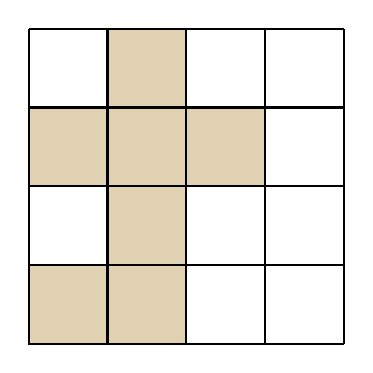
\begin{tikzpicture}
[thick]
\draw (0,0) grid (4,4);
\draw[fill=red!60!green!30!] (1,3) rectangle ++(1,1);
\draw[fill=red!60!green!30!] (1,2) rectangle ++(1,1);
\draw[fill=red!60!green!30!] (1,1) rectangle ++(1,1);
\draw[fill=red!60!green!30!] (1,0) rectangle ++(1,1);
\draw[fill=red!60!green!30!] (0,0) rectangle ++(1,1);
\draw[fill=red!60!green!30!] (0,2) rectangle ++(1,1);
\draw[fill=red!60!green!30!] (2,2) rectangle ++(1,1);
\end{tikzpicture}
\end{figure}
\end{flushleft}

\subsection{Depth Fist Search}

\begin{itemize}
\item To indicate a cell $G[x][y]$ is visited, we can change the value of this cell to a different value like 2.
\item This problem is to find the perimeter. For current cell $G[x][y]$, if it is surrounded by water, the perimeter will be 4. we check its four adjacent cells. If any one of them is also an island (either the value is 1 or 2), decrements the perimeter.
\item We recursively compute for any adjacent island that has not been visited.
\end{itemize}

\setcounter{lstlisting}{0}
\begin{lstlisting}[style=customc, caption={DFS}]
int islandPerimeter( vector<vector<int>>& grid )
{
    int R = static_cast<int>( grid.size() );
    int C = static_cast<int>( grid[0].size() );

    int ans = 0;

    for( int r = 0;  r < R; ++r )
    {
        for( int c = 0; c < C; ++c )
        {
            if( grid[r][c] == 1 )
            {
                dfs( grid, r, c,  ans );
                break;
            }
        }
    }

    return ans;
}

void dfs( vector<vector<int>>& G, int r, int c,  int& len )
{
    //set to 2 to indicate this island is seen before
    G[r][c] = 2;

    int R = static_cast<int>( G.size() );
    int C = static_cast<int>( G[0].size() );

    int dr[4] = {0, -1, 0, 1};
    int dc[4] = {1, 0, -1, 0};

    //If this island is sorrouding by water
    //the perimeter is 4
    //it will be changed if we find adjacent islands
    int p = 4;

    for( int i = 0; i < 4; ++i )
    {
        int nr = r + dr[i];
        int nc = c + dc[i];

        if( ( nr < 0 ) || ( nc < 0 ) || ( nr >= R ) || ( nc >= C ) )
        {
            continue;
        }

        if( G[nr][nc] == 2 )
        {
            //This is also an island
            //will not count the common edge
            --p;
            continue;
        }

        if( G[nr][nc] == 1 )
        {
            //This is also an island
            //will not count the common edge

            --p;
            dfs( G, nr, nc, len );
        }


    }

    len += p;
}
\end{lstlisting}